\section{Programme de construction (6 points)}

Suivre les instructions ci-dessous :
\begin{questions}

		\question[1] Tracer deux droites $(d)$ et $(d_1)$ sécantes en $A$.
		
		\question[1] Placer un point $B$ sur $(d_1)$, tel que $AB$ = 6 cm.
		
		\question[1] Placer un point $C$ tel que $C \in [AB)$ et $C \notin [AB] $.
		
		\question[1] Placer un point $D$ tel que $D \notin (AB)$.
		
		\question[1] Tracer la droite $(d_2)$ perpendiculaire à $(AB)$ passant par $D$.
		
		\question[1] Tracer la droite $(d_3)$, parallèle à $(AB)$ passant par $D$.
		
		\begin{solution}
			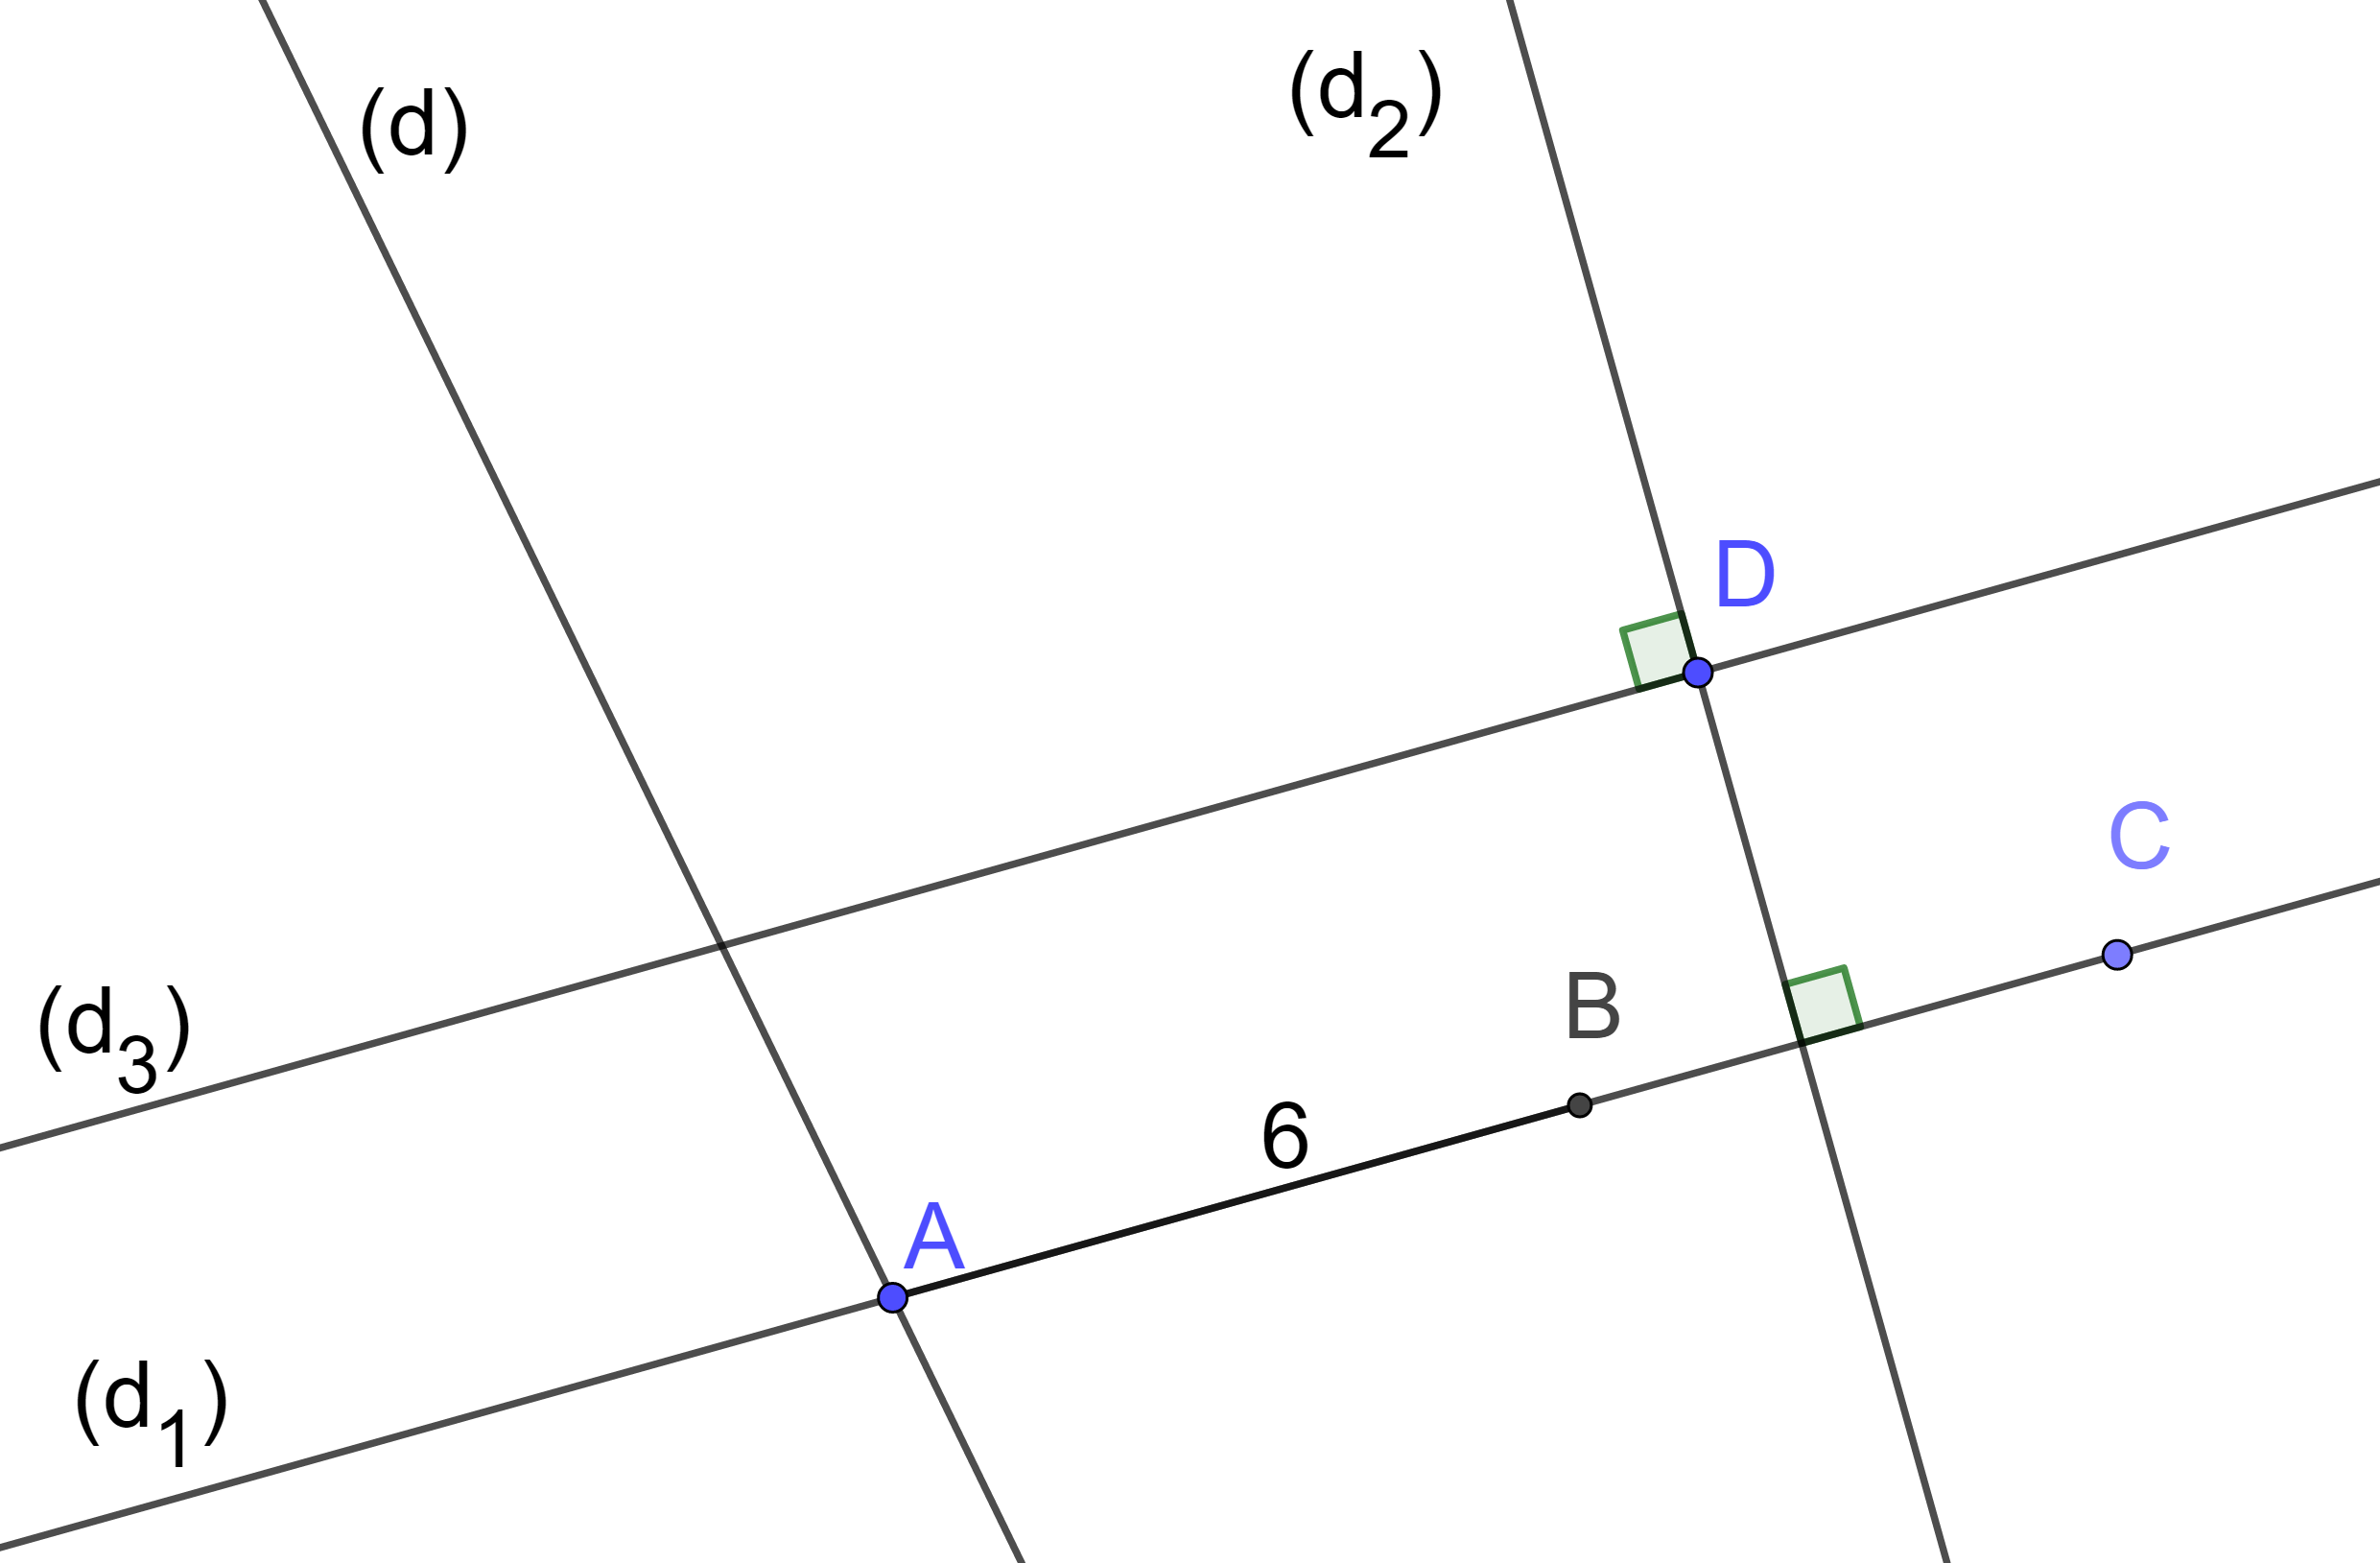
\includegraphics[scale=0.25]{img/exo1_2}
		\end{solution}
	
\end{questions}

